

\section*{Solving 1.1}

\subsection*{Numerical method}
We have system of PDE.

And If used explicit method we obtain 

\begin{equation}\label{explicit}
    u_{i, j} = \frac{1}{2(\delta x^2 + \delta y^2)} \left(\frac{u_{i+1,j} + u_{i-1,j}}{\delta x^2} + \frac{u_{i,j+1} + u_{i,j-1}}{\delta y^2}\right) 
\end{equation}

\begin{figure}[h!]
\centering{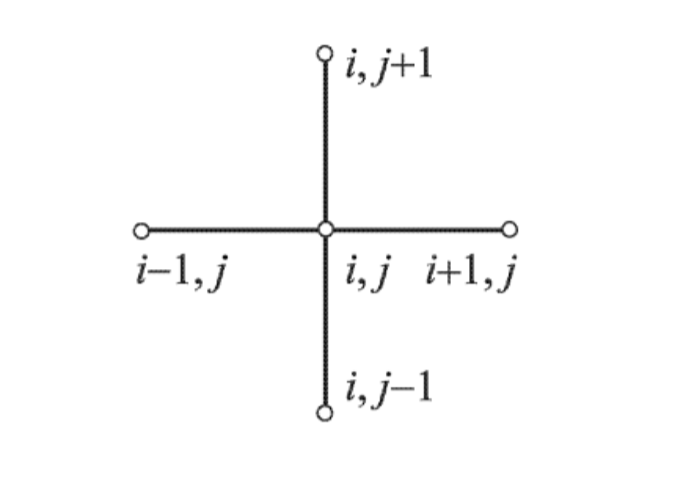
\includegraphics[scale=0.4]{1_1_numerical.png}}
\caption{explicit method}
\end{figure}

Using ($\ref{explicit}$)  for $a=15$ and $b=7$ we obtain (see fig.\ref{Numfig} ) 

\begin{figure}[h]\label{Numfig}
\begin{minipage}[h]{0.49\linewidth}
\center{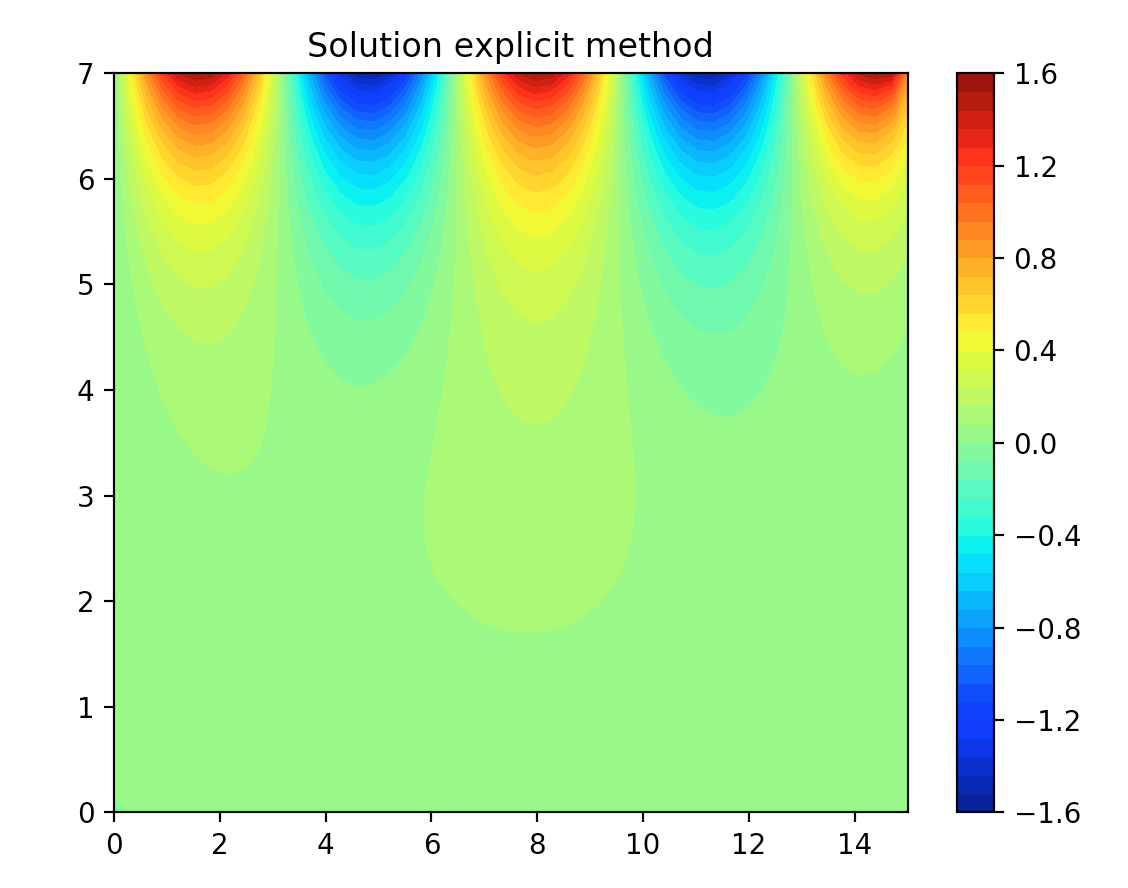
\includegraphics[width=1\linewidth]{NumM_a=15_b=7_t1_1.png} \\ a)}
\end{minipage}
\hfill
\begin{minipage}[h]{0.49\linewidth}
\center{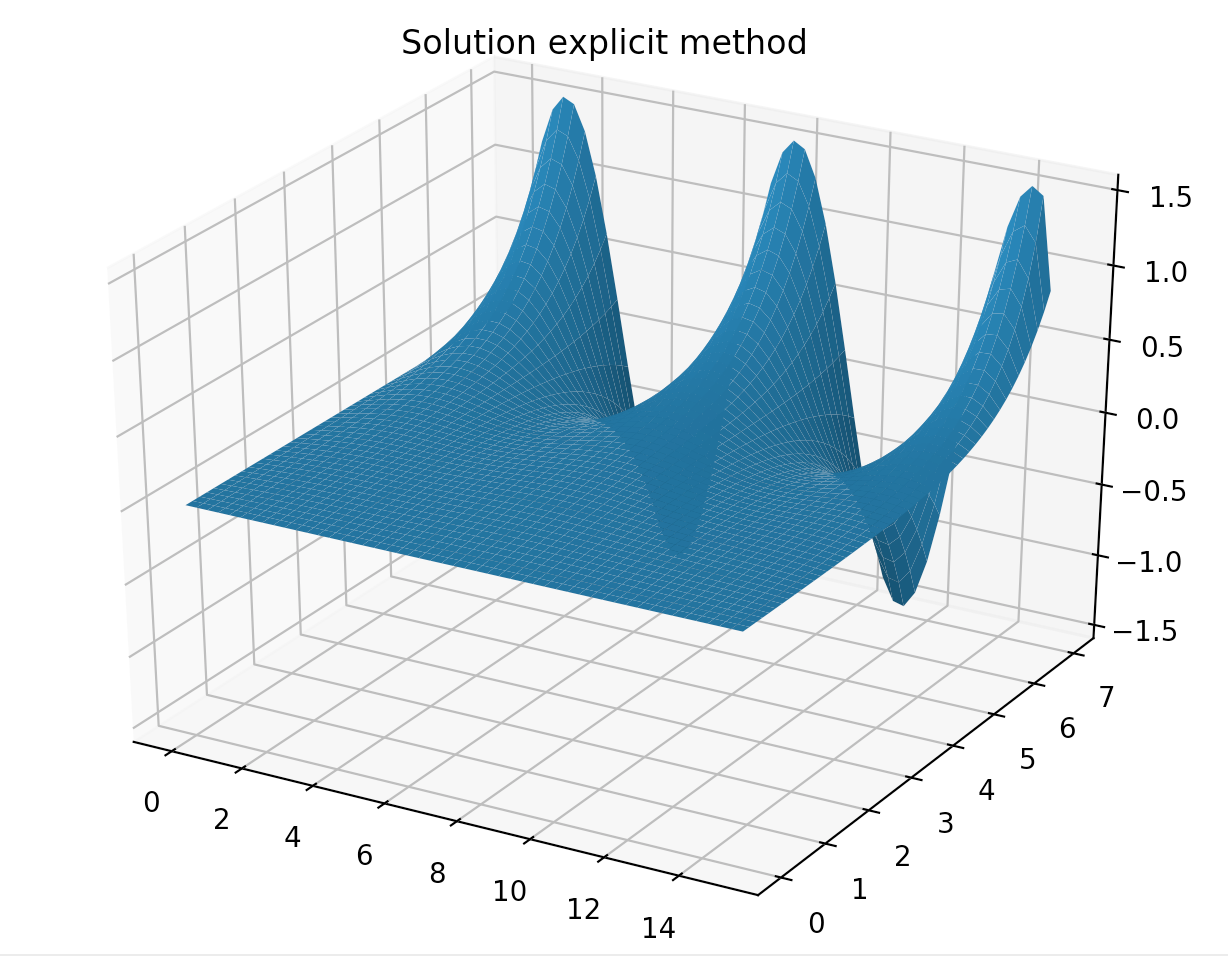
\includegraphics[width=1\linewidth]{NumM3d_a=15_b=7_t1_1 .png} \\ b)}
\end{minipage}
\caption{Numerical Solution (using The Jacobi iterative method) for $a=15$ and $b=7$}
\label{ris:image1}
\end{figure}


\subsection*{Analytical method}

Solving 2D Dirichlet  boundary value problem $(1)$, we obtain 

\begin{equation}\label{an}
    u(x,y) = \frac{xy}{ab} + \frac{2}{\pi} \sum_{n=1}^{\infinity}(-1)^n\left[\left(\frac{b^2 \sinh{\frac{\pi n x }{b}}}{n(b^2 + n^2\pi)}\right)\frac{\sin{\frac{\pi n y}{b}}}{\sinh{\frac{\pi n a }{b}}} +  \left(\frac{a^2 \sinh{\frac{\pi n y }{a}}}{n(a^2 - n^2\pi)}\right)\frac{\sin{\frac{\pi n x}{a}}}{\sinh{\frac{\pi n b }{a}}}\right]
\end{equation}

Using ($\ref{an}$)  for $a=15$ and $b=7$ we obtain (see fig.\ref{Analfig} )

\begin{figure}[h]\label{Analfig}
\begin{minipage}[h]{0.49\linewidth}
\center{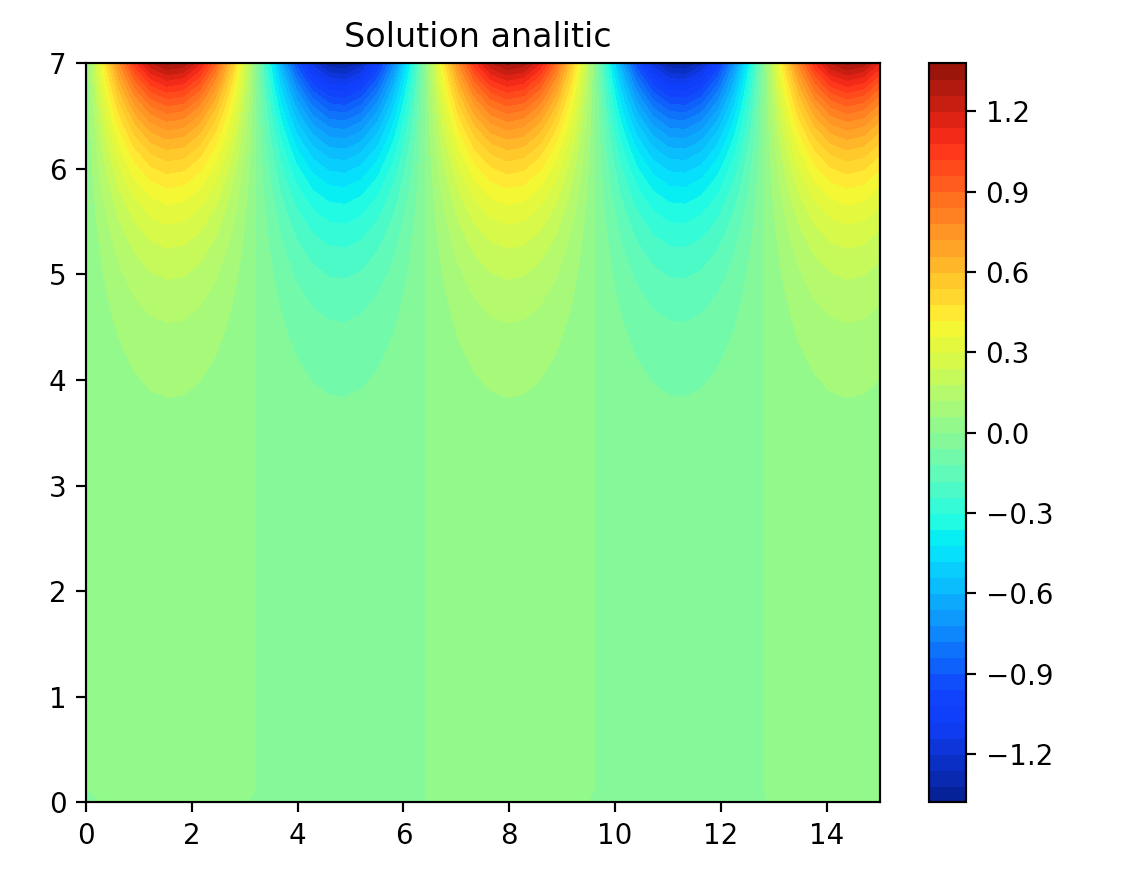
\includegraphics[width=1\linewidth]{AnalM_a=15_b=7_t1_1.png} \\ a)}
\end{minipage}
\hfill
\begin{minipage}[h]{0.49\linewidth}
\center{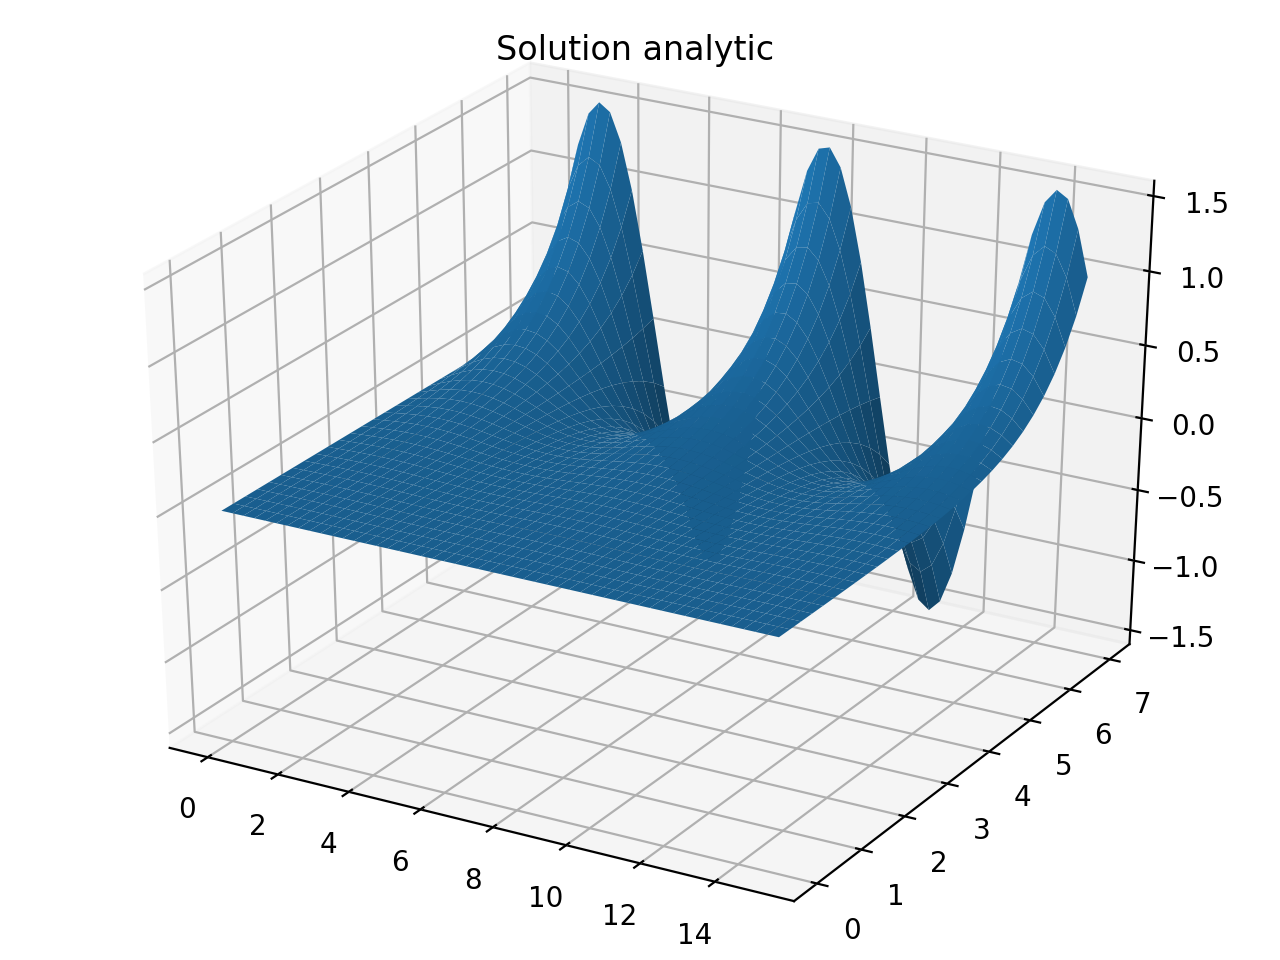
\includegraphics[width=1\linewidth]{AnalM3d_a=15_b=7_t1_1.png} \\ b)}
\end{minipage}
\caption{Analytical Solution  for $a=15$ and $b=7$}
\label{ris:image1}
\end{figure}


